\section{Grues de chantier (3 points)}\label{grues}

Les grues permettent de déplacer de lourdes charges sur un chantier. On s'intéresse à la charge soulevée par la grue.

\begin{questions}
	\question Avec quels objets ou (quels corps) la charge est-elle en interaction ? Préciser à chaque fois le type d'interaction.
		\begin{solution}
			La charge est en interaction de contact avec le câble de la grue et à distance avec la Terre.	
		\end{solution}
	
	\question \'Etablir le diagramme objet-interaction de la charge.
		\begin{solution}
			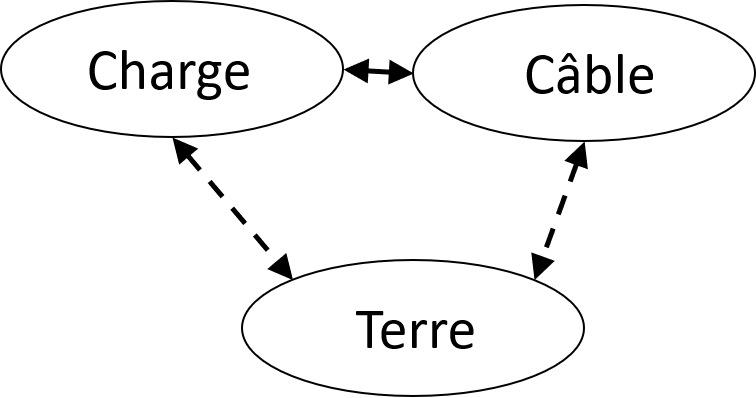
\includegraphics[scale=0.5]{doi_grue}
		\end{solution}
	\question Représenter sur un schéma la force de \num{10000} N exercée par le câble de la grue sur la charge. Préciser l'échelle choisie.
\end{questions}